\section{Introduction}
\section{Synopsis of the Standard Model}
The Standard Model of particle physics is a description of the fundamental constituents of the Universe, as well as the interactions between them.
The model is composed of two main groups of particles, namely the fermions, which possess half-integer quantum spin, and make up all of the 
matter within the Universe, and the gauge bosons, which are of integer quantum spin, and are responsible for mediating forces between the fermions.\\
\\
The fermions can be further classified into two categories of fundamental particles known as quarks and leptons. There exist six distinct 'flavours' of quarks, which are
ascribed the names up, down, charm, strange, top and bottom, denoted, $u, d, c, s, t$ and $b$ respectively. These are grouped into three 'generations' based on their electromagnetic charge
and mass. Free quarks are never observed in nature due to a principle known as quark confinement, which mandates that these particles (and their antiparticles) should exist as bound states known as baryons and mesons
(which are collectively referred to as hadrons). Quarks can interact via all of the abovementioned forces. The leptons are grouped similarly by flavour, with each generation containing a negatively charged particle and a corresponding neutrino
whose electromagnetic charge is zero, and is, to a large extent, massless. The three different flavours of leptons, in ascending order of their masses, are the electron, muon and tau, denoted $e^{-}, \mu^{-}$, and $\tau^{-}$ respectively. The charged leptons
can only partake in electromagnetic and weak interactions while the neutrinos can only participate in weak processes.\\
\\
Three of the four fundamental forces of nature (i.e. the strong, electromagnetic and weak forces) are accounted for in the Standard Model, as evident through the presence of vector (spin 1) gauge bosons such as the gluon ($g$), photon ($\gamma$), and charged $W$ and neutral $Z$ bosons, 
which mediate the aforementioned forces respectively. The model also describes a spin-0 particle, known as the Higgs boson, which, through the mechanism of spontaneous symmetry breaking, is responsible for the Standard Model particles acquiring their mass. A spin-2, massless boson, known as the graviton
has also been hypothesised as a mediator of the gravitational force. However, there is no experimental evidence of this to date. Figure \ref{StandardModel} provides a visual summary of the model that has been described above.\\
\\
\begin{figure}[h!]
    \centering
    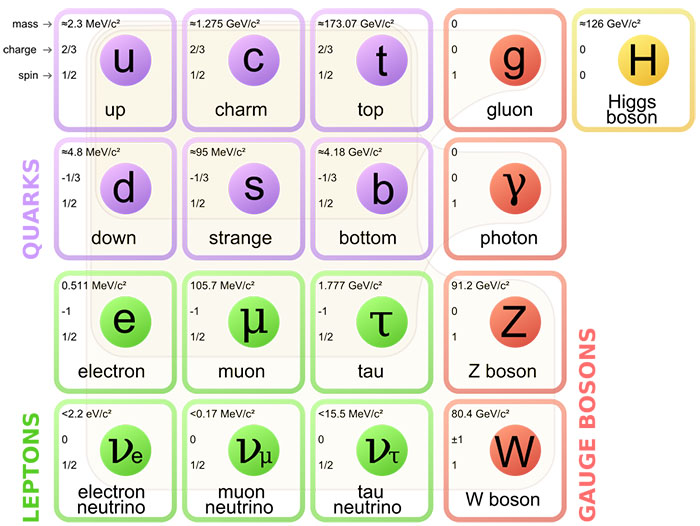
\includegraphics[scale = 0.35]{StandardModel.jpg}
    \caption{The particles of the Standard Model, grouped based on their quantum spin into gauge bosons and fermions (particles that make up all matter).The fermions are further divided into quarks and leptons which are fundamental, and can partake in various interactions that are mediated by the gauge bosons corresponding to each of the three fundamental forces described by the model. The Higgs boson is also included, and is responsible for all of the particles acquiring their mass.}
    \label{StandardModel}
\end{figure}
Despite providing a comprehensive description of the fundamental components of nature and the force acting between these, the Standard Model is subject to numerous limitations, the most prominent of which is its inability to account for the gravitational force. Furthermore, the nature of dark matter and dark energy, which account for
a large proportion of the matter in the Universe, is not fully understood, and remains an area of ongoing research. A more subtle limitation, however, pertains to a phenomenon known as CP violation and the absence of experimental evidence of this in the strong force, despite being theoretically permissible by the quantum field theory of this force,
known as quantum chromodynamics (QCD). This is known as the Strong CP problem and forms the basis for motivating particles such as the axion, as well as Axion-Like Particles (ALPs), both of which are described in further detail in the sections that follow.
\section{CP Violation}
The principle of symmetry (i.e. the invariance of a physical system under a transformation) is significant in the study of particle physics. Two symmetries that are of particular interest are those of charge conjugation, denoted $C$, and parity, denoted $P$. Charge conjugation is a transformation wherein particles within a physical system are interchanged with
their antiparticles, while parity refers to the inversion of spatial coordinates of a physical system, as illustrated in Figure \ref{ParityTransformation} below
\begin{figure}[h]
    \centering
    \begin{subfigure}{0.5\textwidth}
        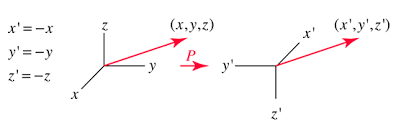
\includegraphics[]{ParityTransformation.png}
        \caption{An illustration of the parity transformation $P$, corresponding
        to the inversion of spatial coordinates in a physical system}
        \label{fig:first}
    \end{subfigure}
    \hfill
    \begin{subfigure}{0.5\textwidth}
        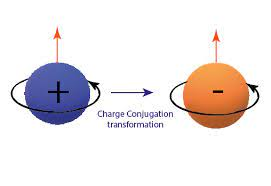
\includegraphics[]{ChargeConjugation.jpg}
        \caption{The Charge conjugation transformation $C$, which interchanges particles in a physical system with their corresponding antiparticles.}
        \label{fig:second}
    \end{subfigure}
    \hfill
\end{figure}\\
The combination of the abovementioned transformations is referred to as $CP$, and its violation is of particular interest as it provides a possible explanation for the abundance of matter over antimatter in the Universe. CP symmetry has been observed to be preserved in electromagnetic interactions, whilst being violated in weak interactions, as demonstrated by 
a study of the decay of neutral kaons by Cronin and Fitch in 1964. While the theory of QCD permits the violation of this symmetry in the strong force, there is no experimental evidence of processes that violate this symmetry. This is referred to as the Strong CP problem, and is essential for the theoretical motivation behind axions and ALPs.
\subsection{The Strong CP Problem}
The two discrete symmetries that are essential to the motivation of the Strong CP problem are charge conjugation, $C$, and parity (i.e. an inversion of spatial coordinates), $P$. While each
of these symmetries can be individually violated by various physical phenomena, their combination CP is known to be conserved in both the strong and electromagnetic interactions, whilst being violated by weak interactions. The strong CP problem arises from the theory pertaining to QCD, which
permits such a violation. Despite this, however, such a process has not been experimentally observed. One can examine the QCD Lagrangian in Equation \ref{QCD_Lagrangian} below, which has been written to include the CP violating terms
\begin{equation}\label{QCD_Lagrangian}
    \mathcal{L}_{QCD} = -\frac{1}{4}G_{\mu\nu}G^{\mu\nu}-\frac{g_{s}^{2}\theta}{32\pi^{2}}G_{\mu\nu}\tilde{G}^{\mu\nu}+\bar{\psi}(i\gamma^{\mu}D_{\mu}-me^{i\theta'\gamma_{5}})\psi
\end{equation}
The terms $\theta$ is CP violating
% Describe the Strong CP problem here and hint towards it's resolution
\subsection{Axions}
\subsection{Experimental Searches for Axions}
\subsection{Axion Like Particles (ALPs)}
\subsection{The $B\rightarrow K^{*}A, A\rightarrow\gamma\gamma$ Decay Process}
\section{Flavour Changing Neutral Currents} 
\section{Electroweak Penguin Decays} 
